\documentclass[tikz,border=3pt]{standalone}
\usepackage{amsmath,amssymb}
\usetikzlibrary{arrows.meta,positioning,calc,fit,backgrounds,decorations.pathreplacing,shapes.geometric}

\begin{document}
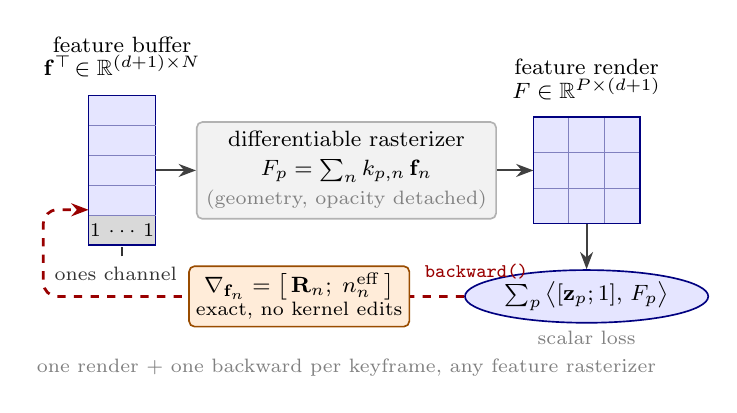
\begin{tikzpicture}[
  font=\footnotesize,
  box/.style={draw, rounded corners=2pt, line width=0.6pt},
  fwd/.style={-{Stealth[length=2.2mm]}, line width=0.7pt, black!75},
  bwd/.style={-{Stealth[length=2.2mm]}, line width=1.0pt, red!60!black, dashed},
]

% ---------- LEFT: feature buffer (tall thin matrix) ----------
\def\bufL{-0.425}\def\bufR{0.425}\def\bufT{1.05}\def\bufB{-0.85}
\fill[blue!10] (\bufL,\bufB) rectangle (\bufR,\bufT);
\fill[gray!30] (\bufL,\bufB) rectangle (\bufR,-0.47);                 % ones channel row
\draw[blue!50!black, line width=0.6pt] (\bufL,\bufB) rectangle (\bufR,\bufT);
\foreach \y in {0.67,0.29,-0.09,-0.47}
  \draw[blue!50!black!50, line width=0.3pt] (\bufL,\y) -- (\bufR,\y);
\node at (0,-0.66) {\scriptsize $1\,\cdots\,1$};
\node[align=center, anchor=south] at (0,1.16)
  {feature buffer\\[-1pt] $\mathbf{f}^{\top}\!\in\mathbb{R}^{(d+1)\times N}$};
% ones-channel callout
\node[anchor=north, text=gray!40!black] (ones) at (-0.08,-1.0) {\scriptsize ones channel};
\draw[gray!40!black, line width=0.4pt] (0,-0.99) -- (0,-0.87);

% ---------- MIDDLE: differentiable rasterizer ----------
\node[box, fill=gray!10, draw=gray!60, align=center] (rast) at (2.85,0.1)
  {differentiable rasterizer\\[1pt]
   $F_p=\sum_n k_{p,n}\,\mathbf{f}_n$\\[1pt]
   {\scriptsize\textcolor{gray}{(geometry, opacity detached)}}};

% ---------- RIGHT: feature render (3x3 grid) ----------
\def\gx{5.9}
\fill[blue!10] (\gx-0.675,-0.575) rectangle (\gx+0.675,0.775);
\foreach \i in {1,2}{
  \draw[blue!50!black!50, line width=0.3pt] (\gx-0.675+0.45*\i,-0.575) -- (\gx-0.675+0.45*\i,0.775);
  \draw[blue!50!black!50, line width=0.3pt] (\gx-0.675,-0.575+0.45*\i) -- (\gx+0.675,-0.575+0.45*\i);}
\draw[blue!50!black, line width=0.6pt] (\gx-0.675,-0.575) rectangle (\gx+0.675,0.775);
\node[align=center, anchor=south] at (\gx,0.875)
  {feature render\\[-1pt] $F\in\mathbb{R}^{P\times(d+1)}$};

% scalar loss node
\node[ellipse, draw=blue!50!black, fill=blue!10, line width=0.6pt, inner sep=1.5pt] (loss) at (\gx,-1.5)
  {\footnotesize $\sum_p\big\langle[\mathbf{z}_p;1],\,F_p\big\rangle$};
\node[text=gray] at (\gx,-2.02) {\scriptsize scalar loss};

% ---------- FORWARD arrows ----------
\draw[fwd] (\bufR,0.1) -- (rast.west);
\draw[fwd] (rast.east) -- (\gx-0.675,0.1);
\draw[fwd] (\gx,-0.575) -- (loss.north);

% ---------- BACKWARD sweep ----------
\draw[bwd, rounded corners=5pt] (loss.west) -| (-1.0,-0.4) -- (\bufL,-0.4);
\node[text=red!60!black] at (4.5,-1.18) {\scriptsize\texttt{backward()}};

% payoff chip (sits on the backward path)
\node[box, fill=orange!15, draw=orange!60!black, align=center, inner sep=2.5pt] at (2.25,-1.5)
  {\footnotesize $\nabla_{\mathbf{f}_n}=\big[\,\mathbf{R}_n;\;n^{\mathrm{eff}}_n\,\big]$\\[-1pt]
   \scriptsize exact, no kernel edits};

% ---------- bottom caption line ----------
\node[text=gray] at (2.85,-2.4)
  {\scriptsize one render $+$ one backward per keyframe, any feature rasterizer};

\end{tikzpicture}
\end{document}
